\documentclass{article}\usepackage{graphicx, color}
%% maxwidth is the original width if it is less than linewidth
%% otherwise use linewidth (to make sure the graphics do not exceed the margin)
\makeatletter
\def\maxwidth{ %
  \ifdim\Gin@nat@width>\linewidth
    \linewidth
  \else
    \Gin@nat@width
  \fi
}
\makeatother

\IfFileExists{upquote.sty}{\usepackage{upquote}}{}
\definecolor{fgcolor}{rgb}{0.2, 0.2, 0.2}
\newcommand{\hlnumber}[1]{\textcolor[rgb]{0,0,0}{#1}}%
\newcommand{\hlfunctioncall}[1]{\textcolor[rgb]{0.501960784313725,0,0.329411764705882}{\textbf{#1}}}%
\newcommand{\hlstring}[1]{\textcolor[rgb]{0.6,0.6,1}{#1}}%
\newcommand{\hlkeyword}[1]{\textcolor[rgb]{0,0,0}{\textbf{#1}}}%
\newcommand{\hlargument}[1]{\textcolor[rgb]{0.690196078431373,0.250980392156863,0.0196078431372549}{#1}}%
\newcommand{\hlcomment}[1]{\textcolor[rgb]{0.180392156862745,0.6,0.341176470588235}{#1}}%
\newcommand{\hlroxygencomment}[1]{\textcolor[rgb]{0.43921568627451,0.47843137254902,0.701960784313725}{#1}}%
\newcommand{\hlformalargs}[1]{\textcolor[rgb]{0.690196078431373,0.250980392156863,0.0196078431372549}{#1}}%
\newcommand{\hleqformalargs}[1]{\textcolor[rgb]{0.690196078431373,0.250980392156863,0.0196078431372549}{#1}}%
\newcommand{\hlassignement}[1]{\textcolor[rgb]{0,0,0}{\textbf{#1}}}%
\newcommand{\hlpackage}[1]{\textcolor[rgb]{0.588235294117647,0.709803921568627,0.145098039215686}{#1}}%
\newcommand{\hlslot}[1]{\textit{#1}}%
\newcommand{\hlsymbol}[1]{\textcolor[rgb]{0,0,0}{#1}}%
\newcommand{\hlprompt}[1]{\textcolor[rgb]{0.2,0.2,0.2}{#1}}%

\usepackage{framed}
\makeatletter
\newenvironment{kframe}{%
 \def\at@end@of@kframe{}%
 \ifinner\ifhmode%
  \def\at@end@of@kframe{\end{minipage}}%
  \begin{minipage}{\columnwidth}%
 \fi\fi%
 \def\FrameCommand##1{\hskip\@totalleftmargin \hskip-\fboxsep
 \colorbox{shadecolor}{##1}\hskip-\fboxsep
     % There is no \\@totalrightmargin, so:
     \hskip-\linewidth \hskip-\@totalleftmargin \hskip\columnwidth}%
 \MakeFramed {\advance\hsize-\width
   \@totalleftmargin\z@ \linewidth\hsize
   \@setminipage}}%
 {\par\unskip\endMakeFramed%
 \at@end@of@kframe}
\makeatother

\definecolor{shadecolor}{rgb}{.97, .97, .97}
\definecolor{messagecolor}{rgb}{0, 0, 0}
\definecolor{warningcolor}{rgb}{1, 0, 1}
\definecolor{errorcolor}{rgb}{1, 0, 0}
\newenvironment{knitrout}{}{} % an empty environment to be redefined in TeX

\usepackage{alltt}
\usepackage{times}
\usepackage{ie07}
\usepackage{hyperref}
\usepackage{amsmath}




\begin{document}


\title{AN OPEN SOURCE TOOL TO ESTIMATE MASS AND EFFICIENCY OF WIND TURBINE POWER TAKE-OFF SYSTEMS}

\authorname{Ozan Keysan, Markus A. Mueller}
\authoraddr{Institute for Energy Systems, University of Edinburgh, EH93JL, U.K.\\
Email: o.keysan@ed.ac.uk}

\maketitle

\keywords
Wind turbine, mass estimation, direct-drive, gearbox, generator

\abstract
This is where the abstract should be placed. It should
consist of one paragraph and a concise summary of the
material discussed in the article below. It is preferable not
to use footnotes in the abstract or the title. The
acknowledgement for funding organisations etc. is placed
in a separate section at the end of the text. We wish you
success with the preparation of your manuscript.

\section{Introduction}

Far offshore wind turbines can help to exploit the wind energy resources that remained untapped so far. These turbines are planned to be installed as floating platforms due to  high water depths (\textgreater 40 m). Reliability and mechanical stability is the most important issues of floating wind turbines. The nacelle mass is critical for the mechanical stability of the platform \cite{Sethuraman2013,Christiansen2011}. A higher mass on the top of the tower increases the center of mass significantly, and this should be balanced with a larger ballast, which increases the installation cost. 

Although, doubly-fed induction generator coupled to a multi-stage gearbox is the most common power take-off (PTO) type for onshore wind turbines; it may not be the most suitable option for a large offshore wind turbine. A direct-drive power take-off systems can be used to eliminate the gearbox, but the mass of a direct-drive generator can be larger than a high-speed power take-off system depending on the power rating and diameter.


In this study, data from manufacturers and literature are collected to predict the  mass and efficiency trend lines for wind turbine components. These equations are used to build an open-source tool that can estimate the mass and efficiency of the total power take-off system. Users can modify the data and models using the tools defined in Appendix-A.

\section{Power Take-Off Components}

The main power take-off components in a wind turbine can be listed as: bearing, shaft, gearbox (if applicable), and generator. 

\subsection{Gearbox}

\subsubsection{Multi Stage Gearbox}

The most common gearbox type used in wind turbines is the three-stage gearbox, which increases the turbine speed to approximately 1500 rpm. Three-stage geraboxes are usually connected to asynchronous generators. 

Data from the following three-stage wind turbine gearbox manufacturers are collected: Bosch-Rexroth\cite{bosch}, Winergy\cite{winergy}, Moventas\cite{Moventas}, Eickhoff\cite{eickhoff}, and General Electric\cite{GE}, and plotted in \autoref{fig:gearbox}. From the figure, it may be seen that the mass of the gearbox is proportional to input torque, which is represented as a linear function in \autoref{3G_gearbox}. 

\begin{knitrout}
\definecolor{shadecolor}{rgb}{0.969, 0.969, 0.969}\color{fgcolor}\begin{figure}[]

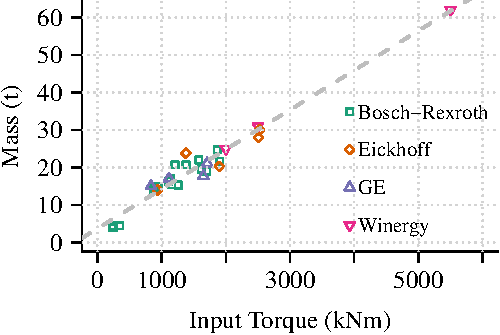
\includegraphics[width=\maxwidth]{figure/gearbox} \caption[Mass of three-stage gearboxes versus torque]{Mass of three-stage gearboxes versus torque.\label{fig:gearbox}}
\end{figure}


\end{knitrout}

\begin{equation}
\text{Mass(t)} = 0.011 \times T_{in} + 3.7
\label{3G_gearbox}
\end{equation}

Multi-stage gearboxes usually consist of two planetary gear stages and an additional high-speed parallel-shaft helical gear stage. In \cite{Hau2005a} it is stated that each planetary gear stages have 1 \% power loss and each helical gear stages have 2 \% power loss. Thus, the efficiency of a three-stage gearbox can be represented as in \cite{Zhang2011a}:

\begin{equation}
  \text{Efficiency(\%)} = 97.0 - \dfrac{P_{in}}{P_{rated}}
\end{equation}

The equation implies that the efficiency of a three-stage gearbox varies from 97 \% at no load to 96 \% at full load.


\subsubsection{Single Stage Gearbox}

Gear ratios up to 15:1 can be achieved using a single stage gearbox \cite{Cotrell2002}. Single-stage gearboxes usually consist of a planetary stage with various numbers of gears depending on the power rating. Single stage gearboxes have fewer gears and bearings than the high-speed gearboxes, which inreased the reliability. Moreover, their efficiencies are higher than 3-stage gearboxes. In \cite{Matveev2011}, the efficiency of a single stage gearbox is given as:

\begin{equation}
  \text{Efficiency(\%)} = 99.5 - \dfrac{P_{in}}{P_{rated}}
\end{equation}

Mass of a single-stage gearbox coupled with medium-speed generator can be approximated as in \cite{Fingersh2006}:

\begin{equation}
	\text{Mass(t)} = 88.3 \times {T_{in}}^{0.774}
\end{equation}

where $T_{input}$ is the input torque in kNm.


\subsection{Structural Components}

\subsubsection{Low Speed Shaft}
Low speed shaft is not a critical component; it connects the main hub to gearbox or generator. Low speed shaft is not required for some drive train options (e.g. integrated bearing type). The mass and the cost of the low speed shaft as a function of the rotor diameter can be expressed as \cite{Fingersh2006}:

\begin{equation}
	\text{Mass (t)} = 1.35 \times {P_{rated}}^{1.44}
\end{equation}

\subsectiion{Main Bearing}

The mass of the main bearing can vary depending on the bearing type. For example, a double-tapered roller bearing for a direct-drive is heavier than a conventional two-point suspension type bearing. To give and idea the mass of a conventional bearing that is connected to a three-stage gearbox can be estimated as \cite{Fingersh2006};

\begin{equation}
	\text{Mass(t)} = 130 \times {P_{rated}}^{1.75}
\end{equation}

\subsection{Hydraulic Systems}

\subsection{Generator}
The generator types covered are induction generator, permanent-magnet generator, synchronous generator and superconducting generator. The cooling method for the generators are also defined (air or water cooled). 
All these data are combined in an open-source design tool. The user can select different PTO systems, and then define the input power and rotational speed The design tool gives the mass and efficiency of the components. Thus, it is very easy for a user to compare different PTO systems and modify the mechanical models based on these estimations. The design tool is built using Matlab GUI. The aim of the study is to publish it as a web application that is open to wind turbine designers. We aim to expand the toolbox for the reliability calculation of the different PTO systems. The design tool will help the designers to compare different PTO systems and select the most suitable option for the specific application.

\begin{knitrout}
\definecolor{shadecolor}{rgb}{0.969, 0.969, 0.969}\color{fgcolor}\begin{figure}[]

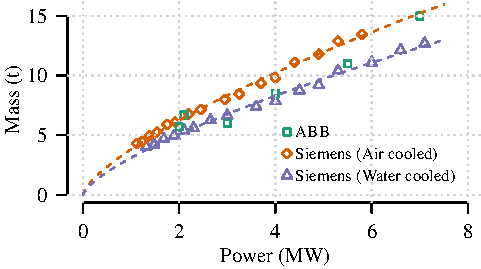
\includegraphics[width=\maxwidth]{figure/induction_generator} \caption[Mass of the induction generator vs torque]{Mass of the induction generator vs torque.\label{fig:induction_generator}}
\end{figure}


\end{knitrout}


\begin{knitrout}
\definecolor{shadecolor}{rgb}{0.969, 0.969, 0.969}\color{fgcolor}\begin{figure}[]

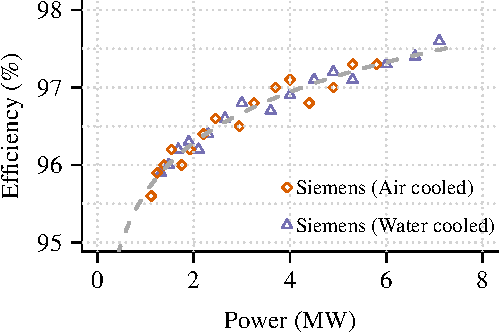
\includegraphics[width=\maxwidth]{figure/induction_generator_eeficiency} \caption[Mass of the induction generator vs torque]{Mass of the induction generator vs torque.\label{fig:induction_generator_eeficiency}}
\end{figure}


\end{knitrout}


\begin{equation}
  \text{Mass}_{air}(t) = 3.91 \times {P_{rated}}^{0.69}
\end{equation}

\begin{equation}
  \text{Mass}_{water}(t) = 3.22 \times {P_{rated}}^{0.68}
\end{equation}

\begin{equation}
\text{Efficiency (\%)} = 95.64 \times {P_{rated}}^{0.01}
\end{equation}



\begin{knitrout}
\definecolor{shadecolor}{rgb}{0.969, 0.969, 0.969}\color{fgcolor}\begin{figure}[]

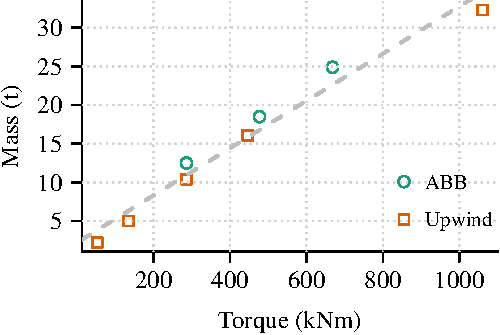
\includegraphics[width=\maxwidth]{figure/plot1gpm} \caption[Mass of the medium speed permanent magnet generator vs torque]{Mass of the medium speed permanent magnet generator vs torque.\label{fig:plot1gpm}}
\end{figure}


\end{knitrout}



\subsection{Direct Drive Synchronous Generator}

\begin{equation}
  \text{Mass(t)} = 0.035 \times {T_{rated}} + 8.9
\end{equation}

\subsection{Permanent Magnet Generator}

\subsubsection{Direct Drive}

\begin{equation}
  \text{Mass(t)} = 0.028 \times {T_{rated}} + 2.8
\end{equation}


\subsubsection{Medium Speed}

\begin{equation}
  \text{Mass(t)} = 0.03 \times {T_{rated}} + 1.5
\end{equation}

As shonw in \autoref{fig:plot1gpm}

The proceedings for IE 07 will contain all the accepted
papers following the peer review process. Authors are
asked to prepare and submit the {\bf PDF} electronic versions
of their full papers according to the instructions below.

\section{Manuscript preparation}
Full papers must be typed in English. The title of the
paper is typed in CAPITAL LETTERS (boldface 18pt)
and centred on the page. The author's name is typed in
capital and lower case bold letters and centred on the
page. Directly under the author's name in capital and
lower case letters and also centred is the author's
affiliation, address, plus e-mail address and fax number of
(at least) the corresponding author. Manuscripts must be
typed single spaced using 10 point characters. Only
Times, Times Roman, Times New Roman and Symbol
fonts are accepted. The text should be typed on an A4
paper (21 cm x 29.7 cm). The paper should have margins
of 2.4 cm from top and bottom and 2 cm from left and
right. Paragraphs are separated by 6 points and with no
indentation. The text of the full papers is written in two
columns and justified. Each column has a width of 8.3 cm
and the columns are separated by a margin of 0.4 cm. The
maximum length of the full paper is 8 pages, of the short
and the demo paper 4 pages. Do not number the pages.
The final format in which the papers will appear on the
CD ROM will be a PDF file. Authors are requested to send
a PDF file of their final paper to be included directly
in the CD ROM.

\subsection{Figures and tables}
Figures and tables should be centred in the column,
numbered consecutively throughout the text, and each
should have a caption underneath it (see for example
Table~\ref{tab1}). Care should be taken that the lettering
is not too small. All figures and tables should be included
in the electronic versions of the full paper.


\begin{table}[htb!]
\begin{center}

\begin{tabular}{|l|l|}
\hline
{\em n} & {\em n!} \\
\hline
1 & 1  \\
2 & 2  \\
3  & 6\\
\hline
\end{tabular}
\end{center}
\caption{\label{tab1}This is an example of a table caption.}
\end{table}

\subsubsection{Equations}
Equations should be typed within the text, centred, and
should be numbered consecutively throughout the text.
They should be referred to in the text as Equation (n).
Their numbers should be typed in parentheses, flush right,
as in the following example.
\begin{equation}
	    PA + A'P - PBR^{-1}B'P + Q  =  0 \enspace.
\end{equation}

\subsubsection{References}
The list of references should be ordered alphabetically
according to the first author surname. All references
should be cited in the text, and using square brackets such
as \cite{ref01} and \cite{ref02}.

\section{Generating a {PDF} file}
The PDF format will be the final format under which the
papers will appear in the {CD ROM}. You {\bf SHOULD}
submit your paper as {PDF} document.

\section{Electronic submission of the full paper}
You should submit your {PDF} file which should adhere to
the above format via the conference paper submission
system.

\section*{Acknowledgements}
The acknowledgement for funding organisations etc.
should be placed in a separate section at the end of the
text. Thank you for your cooperation in complying with
these instructions.

\bibliography{IET_RPG_2013}
\noindent
\bibliographystyle{plain}

\end{document}
